\documentclass[a4paper,12pt]{article}

\usepackage[slovene]{babel}
\usepackage{amsmath, amssymb}
\usepackage{geometry}
\usepackage{graphicx}
\usepackage{tikz}
\usepackage{enumitem}

\geometry{margin=2.5cm}

\title{Matematični delovni list \\ \large 1. letnik srednje šole}
\date{}

\begin{document}

\maketitle


\hrule
\vspace{0.5cm}

\section*{1. naloga}
Poenostavi izraze:
\begin{enumerate}
\item $3x + 5x - 2x = \underline{\hspace{3cm}}$
\item $4(2x - 3) = \underline{\hspace{3cm}}$
\item $(x + 2)(x - 3) = \underline{\hspace{3cm}}$
\item $2x^2 + 3x - x^2 + 4 = \underline{\hspace{3cm}}$
\end{enumerate}

\section*{2. naloga}
Reši enačbe:
\begin{enumerate}
\item $3x + 7 = 22$
\item $5x - 2 = 3x + 10$
\item $2(x + 4) = 3x - 1$
\item $x^2 - 9 = 0$
\end{enumerate}

\vspace{2cm}

\section*{3. naloga}
Dana je funkcija: $y = 2x - 3$

\begin{enumerate}
\item Določi smerni koeficient in začetno vrednost.
\item Izračunaj vrednosti za $x = -1, 0, 2$.
\item Nariši graf funkcije v koordinatnem sistemu:
\end{enumerate}

\begin{center}
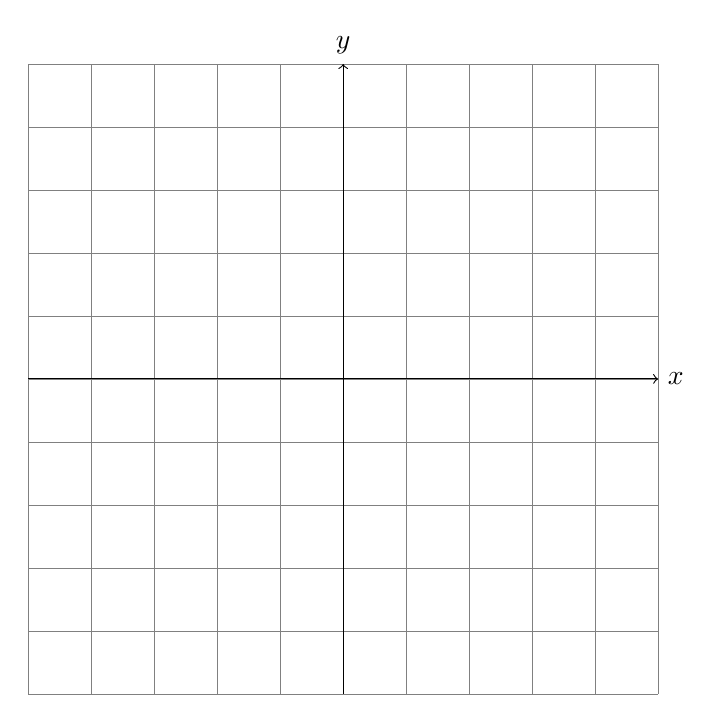
\begin{tikzpicture}[scale=0.8]
\draw[step=1cm,gray,very thin] (-5,-5) grid (5,5);
\draw[->] (-5,0) -- (5,0) node[right] {$x$};
\draw[->] (0,-5) -- (0,5) node[above] {$y$};
\end{tikzpicture}
\end{center}

\section*{4. naloga }
\begin{enumerate}
\item Izračunaj obseg in ploščino trikotnika s stranicami 5 cm, 6 cm, 7 cm.
\item V pravokotnem trikotniku sta kateti 6 cm in 8 cm. Izračunaj hipotenuzo.
\end{enumerate}

\vspace{2cm}

\section*{5. naologa }
Reši sistem:
\[
\begin{cases}
2x + 5y = 7 \\
x - 3y = 1
\end{cases}
\]

\vspace{2cm}

\section*{6. naloga}
\begin{enumerate}
\item Avto prevozi 150 km v 2 urah. Kolikšna je njegova povprečna hitrost?
\item Cena izdelka se poveča za 20\%. Začetna cena je 50 €. Koliko znaša nova cena?
\end{enumerate}

\section*{7. naloga}
\begin{enumerate}
\item Razstavi na faktorje: $x^2 + 5x + 6$
\item Koliko rešitev ima enačba: $x^2 - 4x + 4 = 0$?
\end{enumerate}

\newpage

\section*{8.naloga}

\begin{enumerate}
\item Nariši graf funkcije $y = -x + 2$.

\begin{center}

\begin{tikzpicture}[scale=0.8]
\draw[step=1cm,gray,very thin] (-5,-5) grid (5,5);
\draw[->] (-5,0) -- (5,0);
\draw[->] (0,-5) -- (0,5);
\end{tikzpicture}
\end{center}

\item Nariši graf funkcije $y = x^2$ in označi vrh parabole.

\begin{center}

\begin{tikzpicture}[scale=0.8]
\draw[step=1cm,gray,very thin] (-5,-1) grid (5,9);
\draw[->] (-5,0) -- (5,0);
\draw[->] (0,-1) -- (0,9);
\end{tikzpicture}
\end{center}
\end{enumerate}




\vfill

\hrule


\end{document}